    \subsection{КС грамматика}

\deff{Контекстно-свободная грамматика} 

Концепт в том, что мы задаем выражение через самого себя.

То есть например ПСП задаются:
$$A \xrightarrow{} \varepsilon$$
$$A \xrightarrow{} (A)$$
$$A \xrightarrow{} AA$$
$L \subset \Sigma^*$ - $\Sigma$ - \deff{терминалы}.

$N$ - \deff{нетерминалы} - переменные. $S \in N$ - \deff{стартовый нетерминал}.

$P$ - правило, продукция. $P \subset N \times (N \cup \Sigma)^*$, $P$ - конечная.


$(N \cup \Sigma)^* $ - \deff{сентенциальная форма}.

Будем говорить, что из $\alpha$ выводится за один шаг $\beta$.

$\alpha = \xi A \eta, \beta = \xi\gamma \eta$ и правило $A \xrightarrow{} \gamma \in P$. 

Обозначается $\Rightarrow$. 

\deff{Левосторонний вывод} - заменять только самый левый.

Грамматика $\gamma$ \deff{однозначная}, если $\forall$ слова $\leq 1$ левостор. вывода.

Есть \deff{деревья разбора}:

\begin{center}
   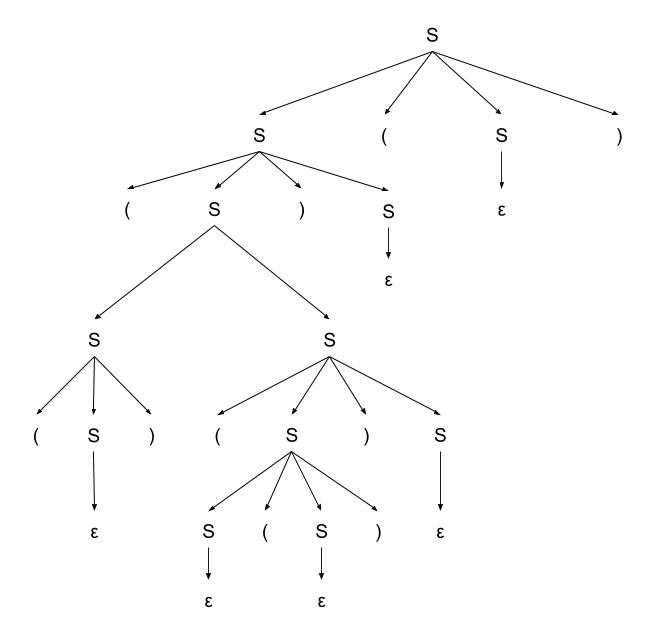
\includegraphics[width=8cm]{assets/11_1_1.png}
\end{center}

Язык $A$ называется \deff{контекстно-свободным}, если его можно задать контекстно свободной грамматикой. 

Грамматика называется \deff{линейной}, если любое правило имеет вид $A \rightarrow \xi B \delta$, или $A \rightarrow \xi$. (не более одного $B$ в любом правиле). А грамматика называется \deff{праволинейной}, если любое правило имеет вид $A \rightarrow \alpha B$ 

\thmm{Теорема:} 

$A$ - регулярный равносильно тому, что $A$ задается праволинейной грамматикой.

\textbf{Доказательство:}

Тривиально.

\textbf{Следствие:} $Reg \subset CF$, $Reg \neq CF$


\deff{Иерархия Хомского.}

\deff{Формальная грамматика} $0$-ого класса - грамматика, но  правила задаются из $N^+$, а не из $N$.


